%Chapter 4 gets to implementation. Explain each pipeline algorithm in sequence
\chapter{Implementation}
\label{chap:implementation}
This chapter will explore in great detail the functionality and implementation of this thesis's pipeline. As a reminder, the pipeline consists of the highlighted elements in Figure~\ref{fig:toplevelpipeline}. Each section of this chapter describes the implementation of one of these functional blocks, as well as a brief exposition on the visualization system. Each section will be accompanied by a figure illustrating the end product of that stage of the pipeline using the same example data.

\section{RGB-D Framework Library}
\begin{figure}[ht]
    \centering
    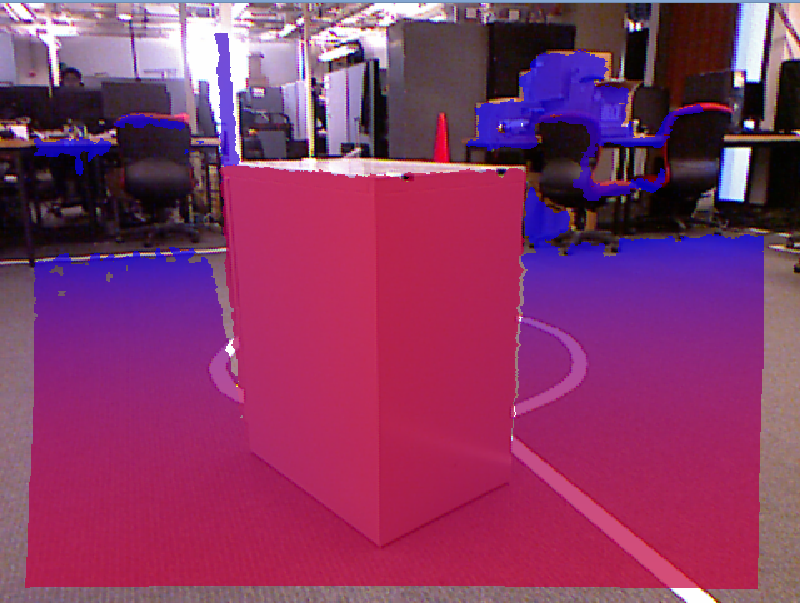
\includegraphics[width=1.0\textwidth]{CabinetDepthOverlay.png}
    \caption{RGB image with depth overlay. Red is closer to the camera, blue is further away. Represents the output of the RGBD Framework}
    \label{fig:rgbdframeworkoutput}
\end{figure}
A crucial component of the pipeline is being able to easily collect RGB-D sensor data from a variety of sources in such a way that the origin of the data is hidden from the remainder of the pipeline. To that end, a highly modular and easily extensible event based framework library was built to seamlessly convert the native data formats and streaming behavior of different sensors. Figure~\ref{fig:rgbdframework} provides an overview of the framework organization. The application code deals directly with four primary classes: RGBDDevice, RGBDFrame, Event Listeners, and FrameLogger. The final output of this framework is a color image and a depth image that are registered in such a way that the pixels have a one-to-one correspondence as shown in Figure~\ref{fig:rgbdframeworkoutput}.
\begin{figure}[ht]
    \centering
    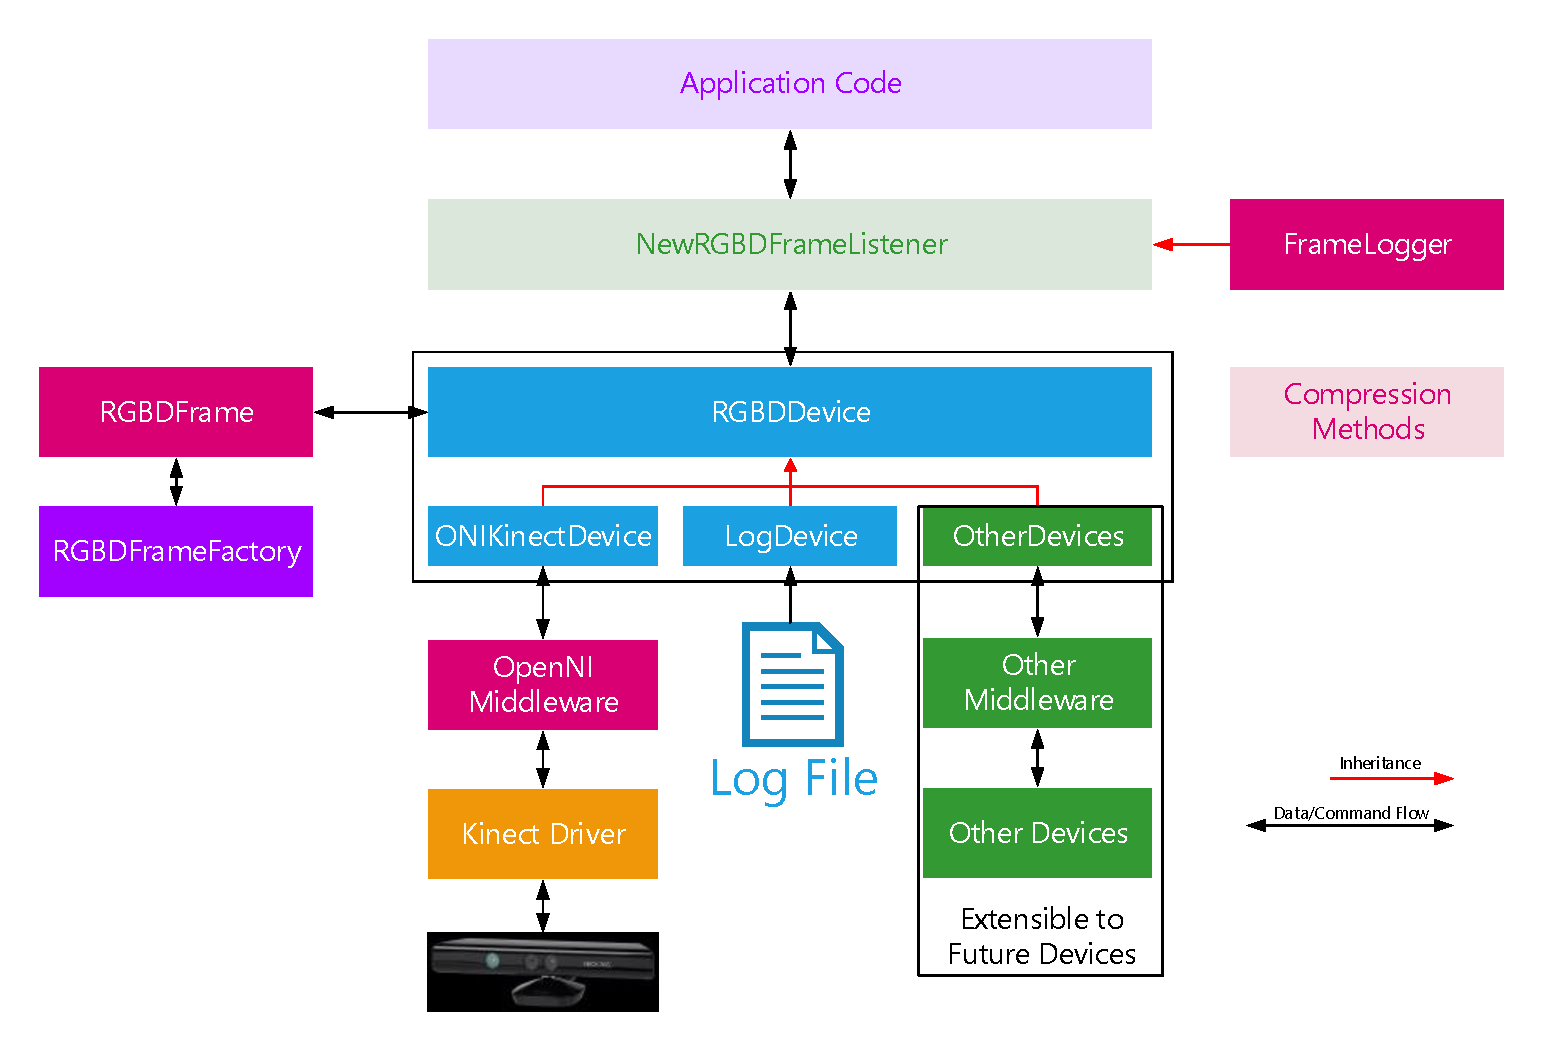
\includegraphics[width=1.0\textwidth]{FrameworkLayout.pdf}
    \caption{RGB-D framework architecture}
    \label{fig:rgbdframework}
\end{figure}
\subsection{RGBDDevice}
The primary interface between the framework and the rest of the application is the abstract class RGBDDevice. RGBDDevice provides an abstract interface including a data stream management API, access to device properties like camera intrinsics and resolution, and event listener registration API. Interfaces for specific devices like the Kinect can be implemented by creating a subclass of RGBDDevice and implementing the abstract methods. The application can then instantiate the desired subclass with device specific initialization parameters and the remainder of the pipeline can be completely agnostic to the underlying nature of the data source, since all RGBDDevices provide the same format RGBDFrame through the same event architecture regardless of the native device formatting. The current framework contains two subclasses: ONIKinectDevice and LogDevice. 
\paragraph{ONIKinectDevice} ONIKinectDevice implements a connection specific to the Microsoft Kinect using OpenNI as middleware. The implementation utilizes OpenNI's event-based interface to receive data from the sensor. Two streams for the color and depth data are created and registered with listeners internal to ONIKinectDevice. When a new depth or color frame is received from OpenNI, the data is copied and repackaged into an RGBDFrame format and a new thread is launched which passes the RGBDFrame to each registered listener. 
\paragraph{LogDevice} LogDevice replays a data log created using the FrameLogger class. Because of the way that the FrameLogger records the data, any device that can be implemented as an RGBDDevice can be recorded and played back using a LogDevice. The framework even allows logging data from a LogDevice. This class allows experiments to be performed very easily on prerecorded data without having to alter the behavior of the pipeline at all.
\subsection{RGBDFrame}
The RGBDFrame is a simple data structure that provides a consistent data formatting for users of the framework. Each frame consists of two managed shared pointers (implemented using boos::shared\_array<T>); one points to the color data and the other points to depth data. Color data is stored in a 24-bit RGB format (1 byte for each component red, green, blue). Depth data is stored in an unsigned 16-bit integer where the least significant bit represents 1mm of resolution (i.e. the value 1024 corresponds to a depth of 1.024m). The frame also has two flags indicating the validity of the depth and color arrays, since not every frame will have both.\par
RGBDFrames are created using a factory design paradigm. The RGBDFrameFactory generates managed pointers which refer to RGBDFrames of a given resolution. Because of the nature of shared pointers, when the last reference to the frames or its component arrays goes out of scope, the frame will delete itself. Because of this, the frames can easily be handed off to the application with no need for the application to be aware of the finer points of the RGBDFramework's memory management scheme. Since roughly 46MB of frame dedicated memory will be allocated every second by the framework, clean, simple memory management is essential.
\subsection{Event Listeners}
The RGBDDevice provides a suite of event listeners that the application code can register listeners for. Four events can be emitted by the RGBDDevice: DeviceConnected, DeviceDisconnected, DeviceMessage, and NewRGBDFrame.
\paragraph{DeviceConnected}
This event is triggered when the underlying device is successfully connected to the RGBDDevice. This usually happens upon success of the RGBDDevice::connect method.
\paragraph{DeviceDisconnected}
This event is triggered when the underlying device is disconnected. This happens either upon calling RGBDDevice::disconnect, or when a fatal communication failure occurs.
\paragraph{DeviceMessage}
This is a special event that allows the device to pass human readable text descriptors to the application for display in the appropriate place. This is useful for debugging or for registering more unique events for a specific device.
\paragraph{NewRGBDFrame}
This event actually transfers the latest RGBDFrame from the sensor to the application. It passes a shared\_ptr to the all registered listeners.
\subsection{FrameLogger}
The FrameLogger class is actually just a special subclass of the NewRGBDFrameListener class. To record the output of any RGBDDevice to a directory, the FrameLogger just needs to be given an output directory using setOutputDirectory. Once that has been done, all that is required to log the output is to call the FrameLogger's startRecording method, which registers the FrameLogger as a NewRGBDFrameListener with the target RGBDDevice. As the logger receives new frames (which can happen in parallel with the primary pipeline), they are tagged with a counter id and saved to the output directory as raw binary files. Some options are also available for data compression.


\section{Filtering and Point Cloud Generation}
\begin{figure}[ht]
    \centering
    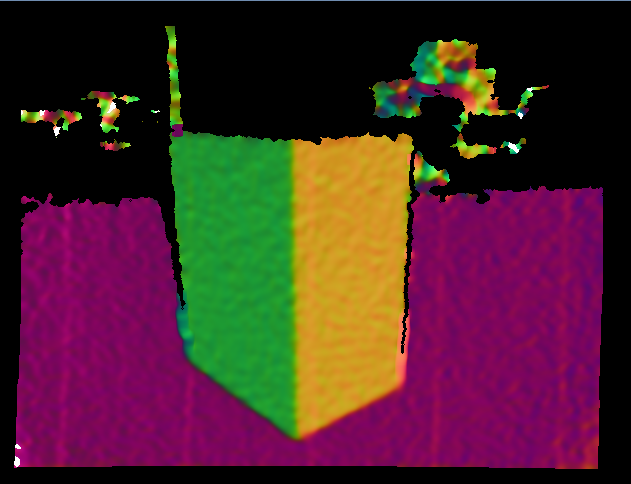
\includegraphics[width=1.0\textwidth]{CabinetNormals.png}
    \caption{Visualization of surface normals, where components of the normal vector are mapped from -xyz to rgb. Example of output from preprocessing stage. }
    \label{fig:filteringoutput}
\end{figure}
Once the raw RGB-D frame has been received, it is pushed to GPU memory. This is the only downstream memory transfer that happens during this entire thesis. Once the memory transfer is complete, the next step is to convert the RGBDFrame format into a floating point representation that is easier to manipulate and perform other preprocessing steps like depth filtering and normal estimation. The data is also converted to a structure of arrays format to improve memory coherence. Figure~\ref{fig:preprocessingdiagram} shows the entire preprocessing system's program flow. 
\begin{figure}[hp]
    \centering
    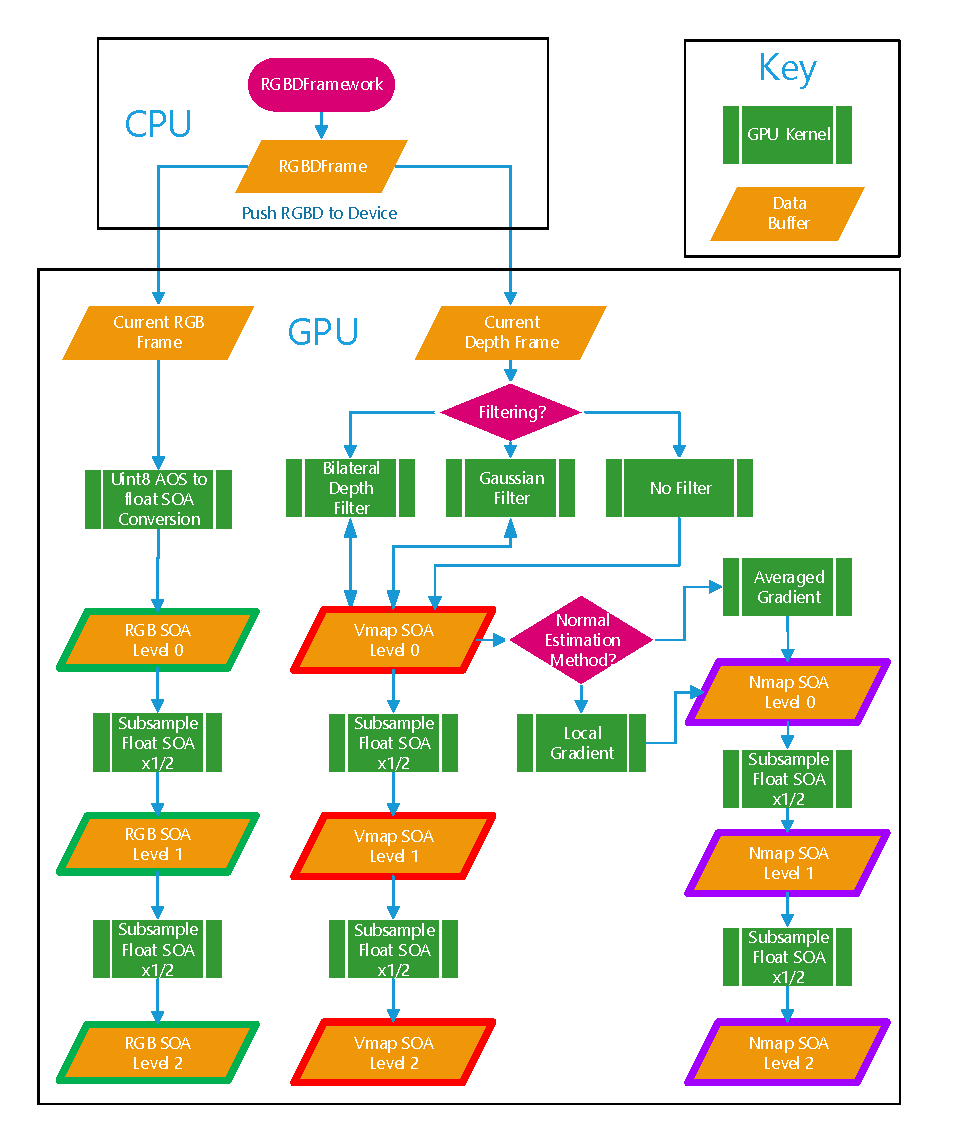
\includegraphics[width=1.0\textwidth]{PreprocessingDiagram.pdf}
    \caption{Preprocessing pipeline diagram.}
    \label{fig:preprocessingdiagram}
\end{figure}
\paragraph{RGB Data Processing} 
The processing for the RGB data is trivial. A kernel converts the 0-255 integer representation of the color data into a 0.0-1.0 floating point representation stored in a structure of arrays (SOA) format for memory coherence. This SOA is then subsampled twice by a factor of two each time, resulting in two additional levels of image resolution. This is useful for later stages in the pipeline that do not require full resolution to function and can therefore be run much faster on the lower resolution image.
\paragraph{Depth Filtering}
The pipeline includes three options for pre-filtering the depth data: no filter, a separable Gaussian filter, and a separable bilateral filter approximation\cite{pham2005separable}. The no filter kernel simply performs the inverse camera projection to convert the depth data into an ordered point cloud stored in the vertex map (VMap) buffer. The formula for this projection is based on the camera intrinsic parameters $\{f_x,f_y,c_x,c_y\}$ and the pixel coordinates $(u,v)$.
$$v_x = (u - c_x) * depth / f_x$$
$$v_y = (v - c_y) * depth / f_y$$
$$v_z = depth$$
Pixels with invalid depth data are stored as NaN to allow easy validation later in the pipeline.\par 
The Gaussian kernel performs the same projection, but also applies a separated implementation of Gaussian filter  $(radius=3 pixels,\sigma=2.0)$ to the depth data before calculating the projection. This helps remove much of the depth quantization and sensor noise that makes normal estimation difficult. However, the Gaussian filter does not preserve edges, so crucial discontinuities in the image are blurred together.\par 
To solve this problem, a bilateral filter is used instead. In addition to the spatial Gaussian term that weights pixels by their screen distance from the center pixel, bilateral filters also apply a Gaussian weight to the difference in intensity. In this way, pixels that have a vastly different depth value will have a lower weight and hard edges can be more easily preserved.\par 
As with the color data, the vertex map is subsampled into a resolution pyramid.
\paragraph{Normal Estimation}
Surface normals are locally estimated for each valid point. Several methods exist for estimating point cloud normals, but the simplest to apply in an ordered image is a gradient based approach. For each point $\vec{p}(x,y)$ Two vectors $\vec{G_x}$ and $\vec{G_y}$ are created from the neighboring points. $$\vec{G_x}(x,y)=\vec{p}(x+1,y)-\vec{p}(x-1,y)$$ $$\vec{G_y}(x,y)=\vec{p}(x,y+1)-\vec{p}(x,y-1)$$
The normalized cross product of these two vectors is then taken to be the point normal. $$\vec{N}(x,y)= \frac{\vec{G_x}(x,y) \times \vec{G_y}(x,y)}{|\vec{G_x}(x,y) \times \vec{G_y}(x,y)|}$$
Since the sign of this normal is ambiguous, all normals are flipped so that they face the viewpoint. The normal faces the viewpoint when the following condition is met: $$\vec{N} \cdot (\vec{p}-\vec{p_eye}) < 0$$
Since in the coordinate frame used at this stage has the eye at the origin looking along the $+z$ axis, this condition can be simplified to: $$\vec{N} \cdot \vec{p} < 0$$
If the estimated normal violates this condition, the negative of the normal is stored.\par
While this simple normal estimate works reasonably well, it can be improved by applying a smoothing filter to the gradient images $G_x$ and $G_y$. A separable Gaussian kernel is applied to each gradient image in turn, and then the cross product is performed. Figure~\ref{fig:filtercompare} compares the various combinations of depth filters and normal estimation methods on the normal estimates. Notice how the Gaussian filter fills in the gaps between the cabinet and the floor, but the bilateral filter shows a very clean break. The final pipeline uses both the bilateral filter and the gradient smoothing techniques.

\begin{figure}[ht]
    \centering
    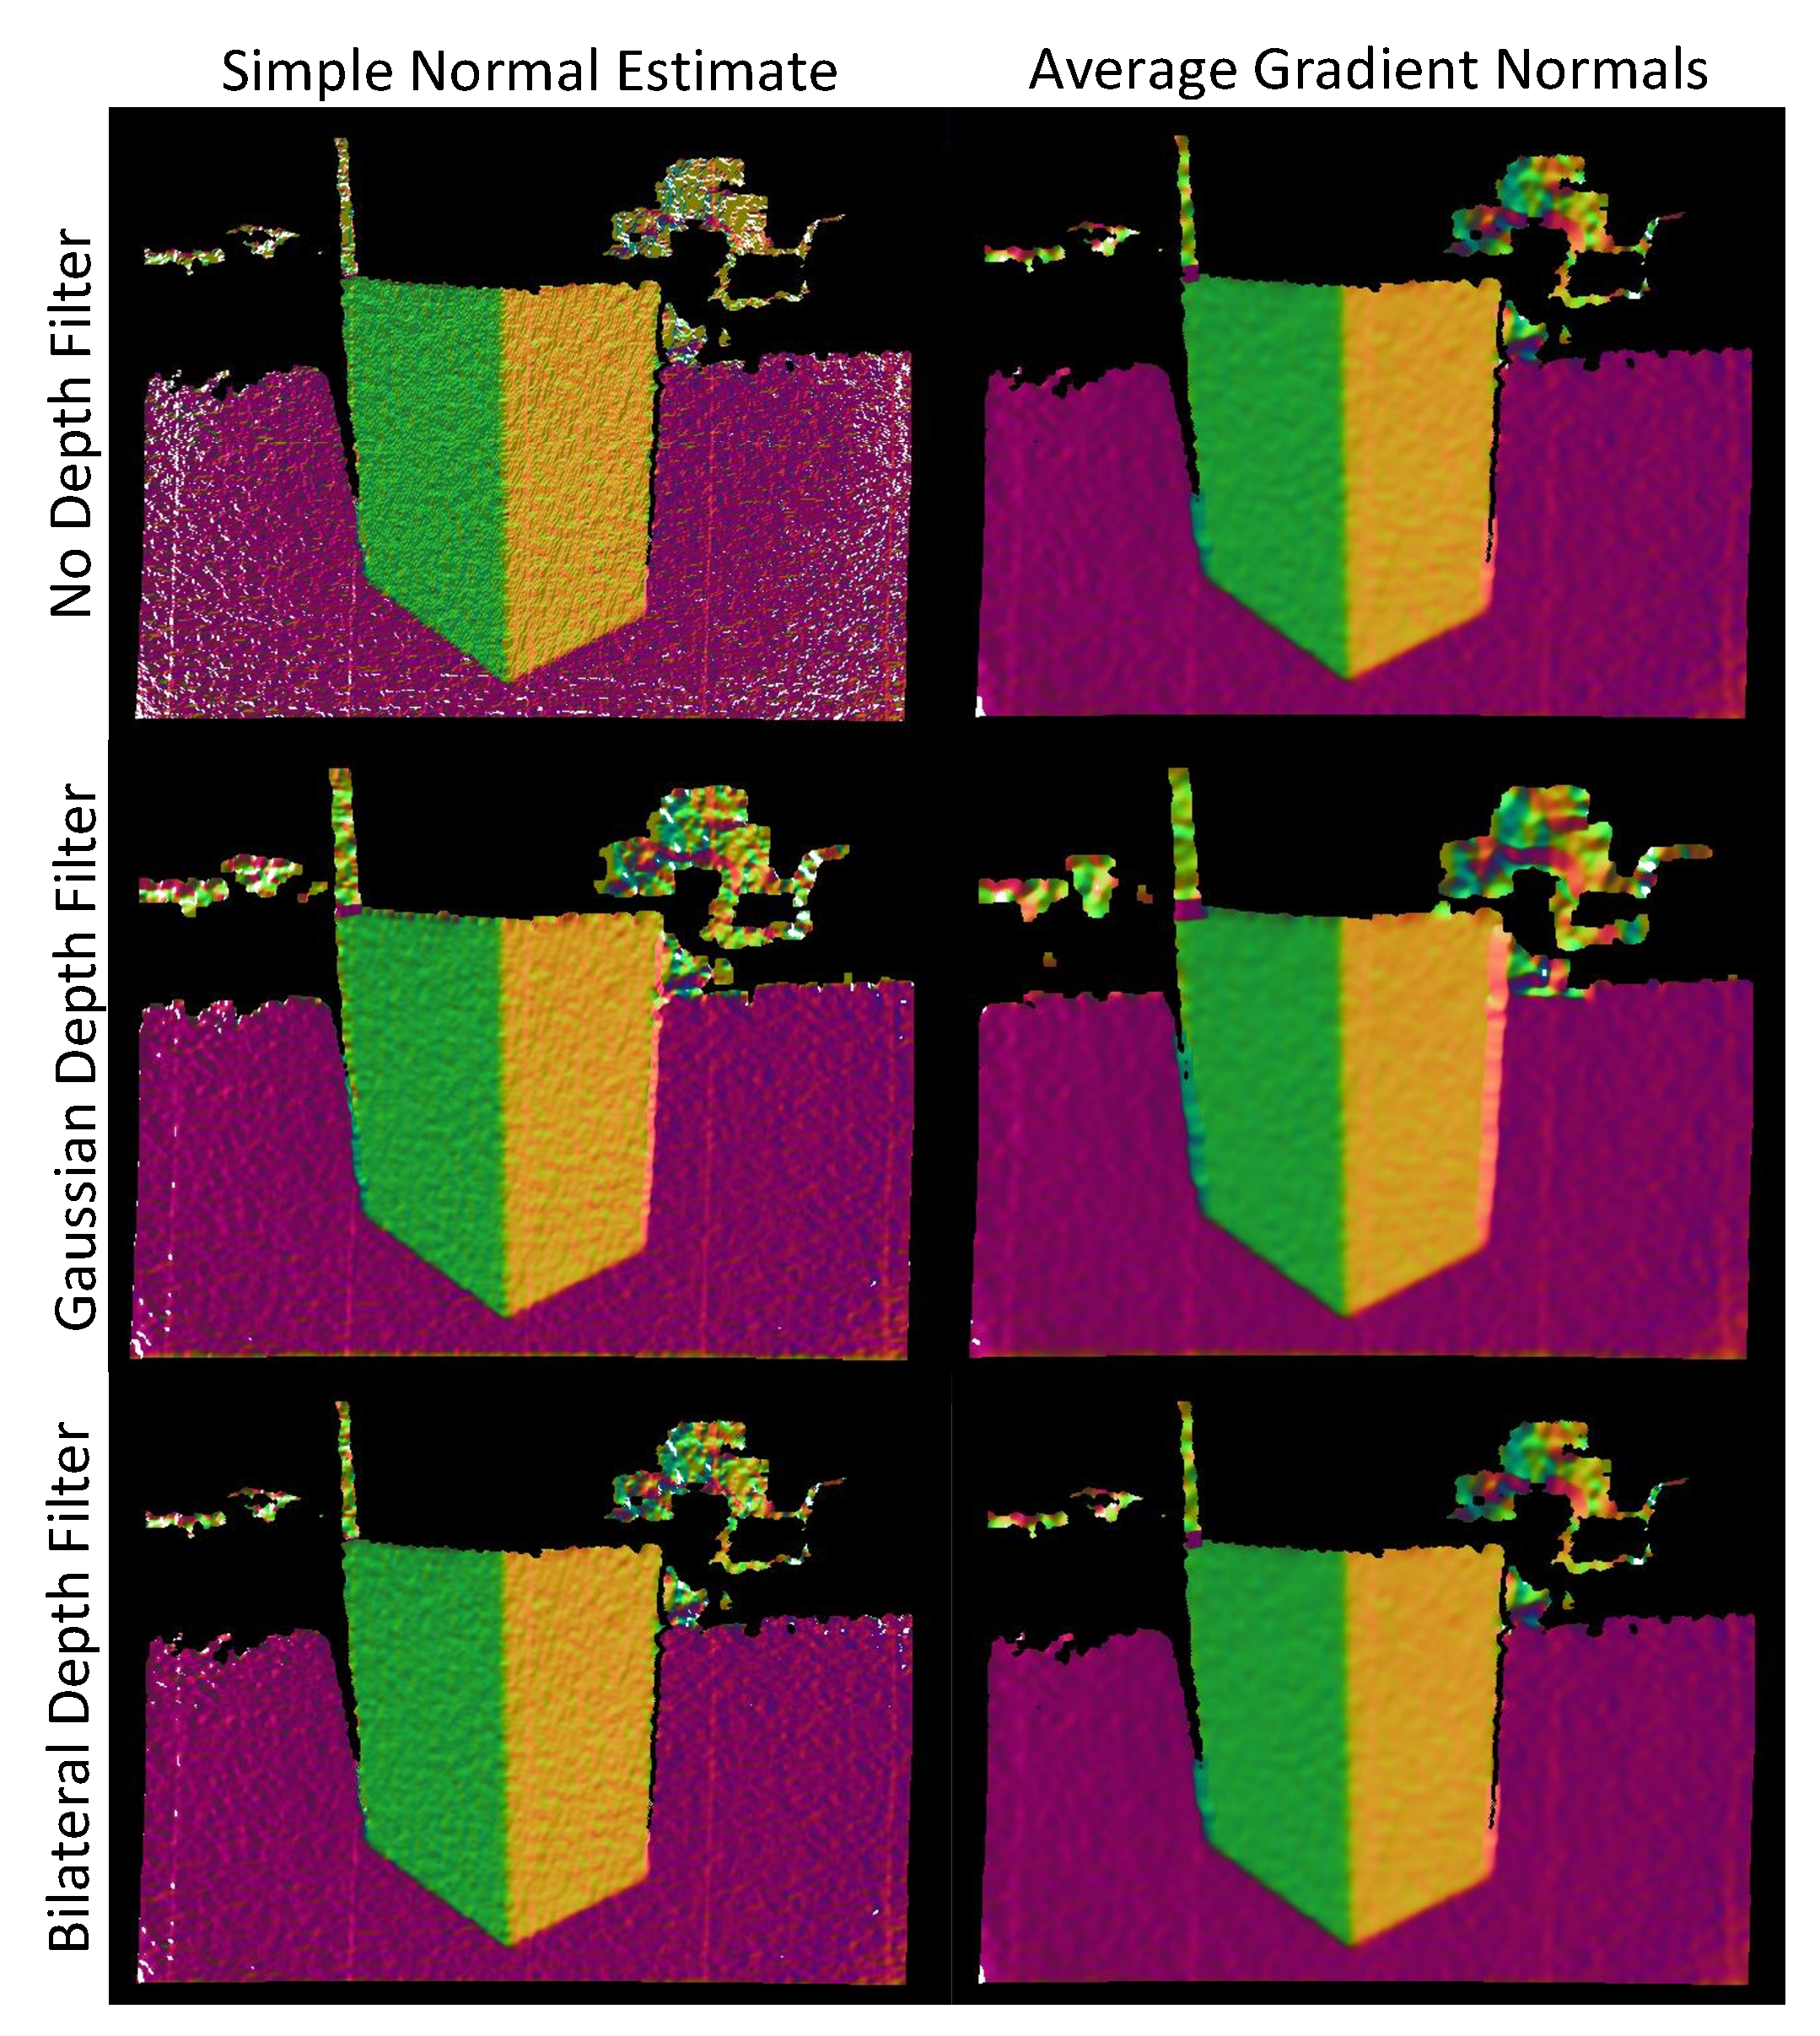
\includegraphics[width=1.0\textwidth]{FilterCompare.pdf}
    \caption{Comparison of the normals estimated using various methods and filters}
    \label{fig:filtercompare}
\end{figure}

\section{Plane Segmentation}
\begin{figure}[ht]
    \centering
    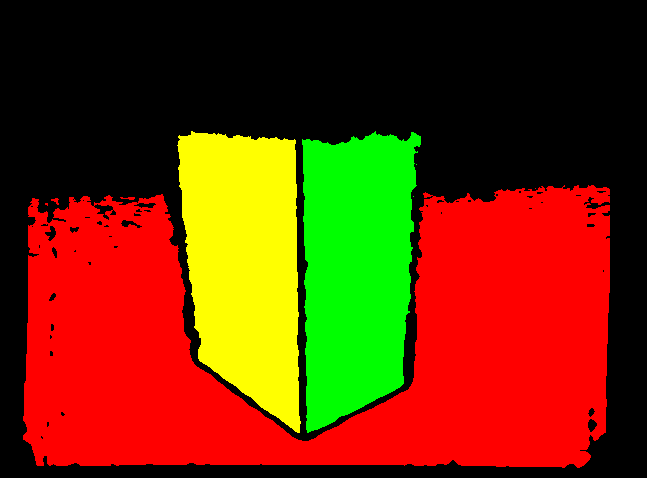
\includegraphics[width=1.0\textwidth]{CabinetPlanes.png}
    \caption{Random colorization of detected planes. Example of output from segmentation stage.}
    \label{fig:segmentationoutput}
\end{figure}


\section{Planar Mesh Generation}
\begin{figure}[ht]
    \centering
    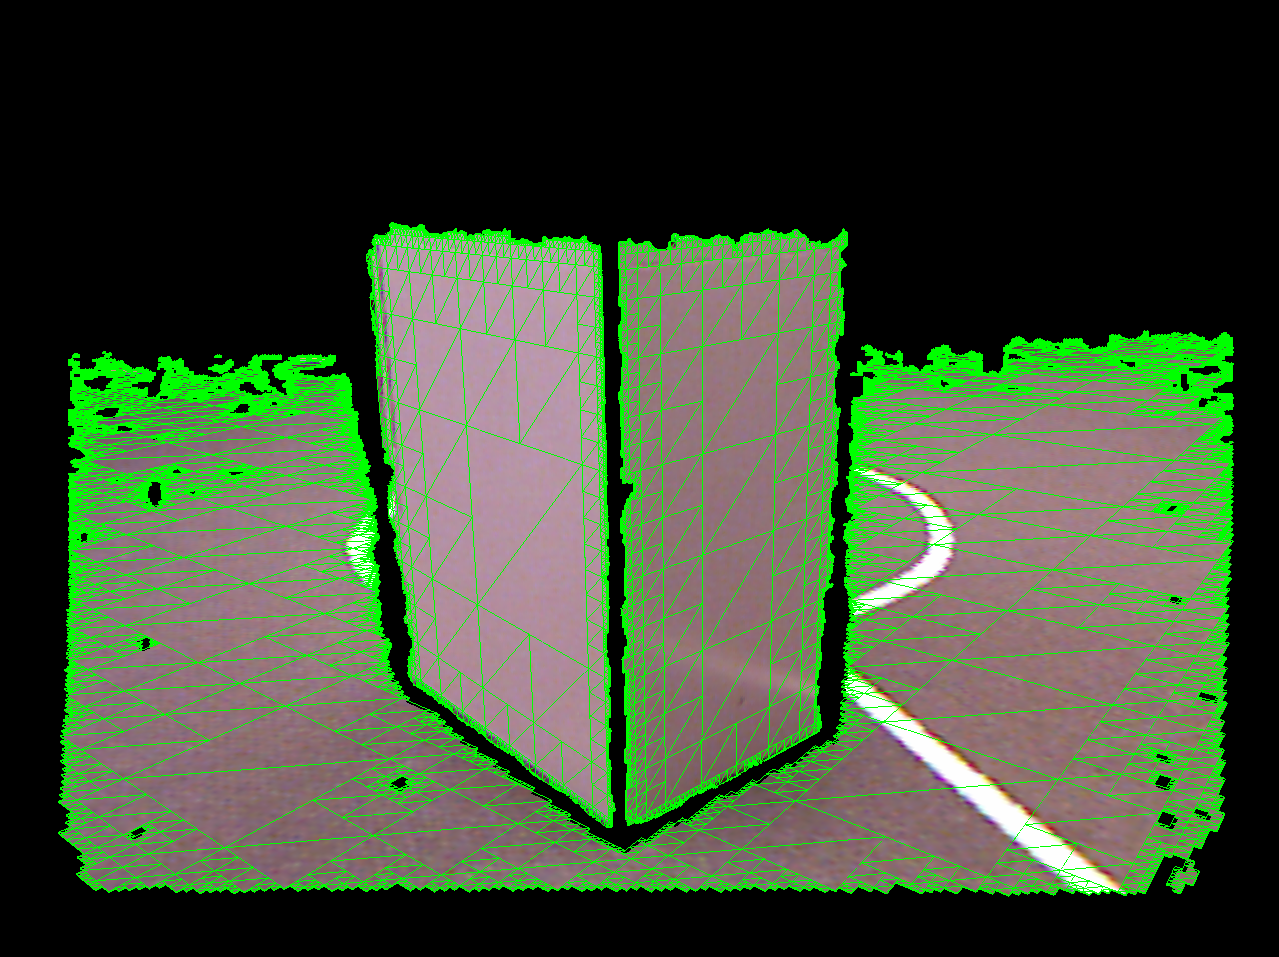
\includegraphics[width=1.0\textwidth]{CabinetMesh.png}
    \caption{Wireframe visualization of the textured mesh. Rendered using the intrinsic parameters of the original camera for direct comparison. Example of output from mesh generation stage.}
    \label{fig:meshoutput}
\end{figure}


\section{Visualization}